\documentclass[a4paper,11pt]{article}
\usepackage{tikz}
\usetikzlibrary{calc,positioning,shapes.geometric,shapes.symbols,shapes.misc}

\tikzset{
	start-end/.style={
		draw,
		rectangle,
		rounded corners,
	},
	input/.style={ % requires library shapes.geometric
		draw,
		trapezium,
		trapezium left angle=60,
		trapezium right angle=120,
	},
	operation/.style={
		draw,
		rectangle
	},
	loop/.style={ % requires library shapes.misc
		draw,
		chamfered rectangle,
		chamfered rectangle xsep=2cm
	},
	decision/.style={ % requires library shapes.geometric
		draw,
		diamond,
		aspect=#1
	},
	decision/.default=1,
	print/.style={ % requires library shapes.symbols
		draw,
		tape,
		tape bend top=none
	},
	connection/.style={
		draw,
		circle,
		radius=5pt,
	},
	process rectangle outer width/.initial=0.15cm,
	predefined process/.style={
		rectangle,
		draw,
		append after command={
			\pgfextra{
				\draw
				($(\tikzlastnode.north west)-(0,0.5\pgflinewidth)$)--
				($(\tikzlastnode.north west)-(\pgfkeysvalueof{/tikz/process rectangle outer width},0.5\pgflinewidth)$)--
				($(\tikzlastnode.south west)+(-\pgfkeysvalueof{/tikz/process rectangle outer width},+0.5\pgflinewidth)$)--
				($(\tikzlastnode.south west)+(0,0.5\pgflinewidth)$);
				\draw
				($(\tikzlastnode.north east)-(0,0.5\pgflinewidth)$)--
				($(\tikzlastnode.north east)+(\pgfkeysvalueof{/tikz/process rectangle outer width},-0.5\pgflinewidth)$)--
				($(\tikzlastnode.south east)+(\pgfkeysvalueof{/tikz/process rectangle outer width},0.5\pgflinewidth)$)--
				($(\tikzlastnode.south east)+(0,0.5\pgflinewidth)$);
			}  
		},
		text width=#1,
		align=center
	},
	predefined process/.default=1.75cm,
	man op/.style={ % requires library shapes.geometric
		draw,
		trapezium,
		shape border rotate=180,
		text width=2cm,
		align=center,
	},
	extract/.style={
		draw,
		isosceles triangle,
		isosceles triangle apex angle=60,
		shape border rotate=90
	},
	merge/.style={
		draw,
		isosceles triangle,
		isosceles triangle apex angle=60,
		shape border rotate=-90
	},
}

\begin{document}
	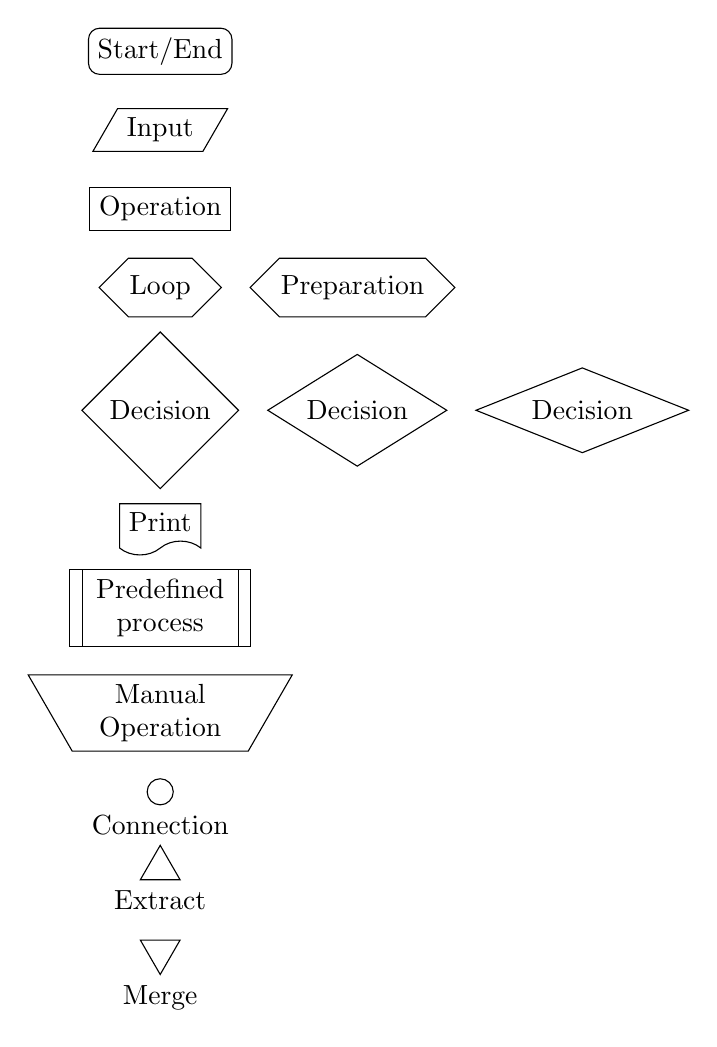
\begin{tikzpicture}
		\node[start-end] (start) {Start/End};
		\node[below of=start,input](inp){Input};
		\node[below of=inp,operation] (op) {Operation};
		\node[below of=op,loop] (lp) {Loop};
		\node[right= 10pt of lp,loop=1.6] (lp2) {Preparation};
		\node[below= 5pt of lp,decision] (dec) {Decision};
		\node[right= 10pt of dec,decision=1.6] (dec2) {Decision};
		\node[right= 10pt of dec2,decision=2.5] (dec3) {Decision};
		\node[below= 5pt of dec,print] (pr) {Print};
		\node[below= 10pt of pr,predefined process] (prproc) {Predefined process};
		\node[below= 10pt of prproc,man op] (manop) {Manual Operation};
		\node[below of=manop,connection, label=below:Connection] (con) {};
		\node[below of=con,extract, label=below:Extract] (extr) {};
		\node[below of=extr,merge, label=below:Merge] (mrg) {};
	\end{tikzpicture}
\end{document}